\subsection{Subsystem Testing}
% talks about different rigorous methods of testing the system

%\noindent FOV directivity test for range sensors, depression angle test, incoming data stream test.\\
% raise alerts if range threshold is crossed
% object detection test - range updates continuously and raises flag or interrupt if crosses below a threshold of danger
% - passing obstacle (confirm margin of safety)
% - moving obstacle
\subsubsection{Detection FOV Threshold} \label{ardumatlab}
\noindent The first test for the obstacle detection subsystem is straightforward. It will consist of the sensor readings code uploaded to the microcontroller, connected to a laptop which rests on the seat of the rollator. The serial plotter will be open and we aim to observe changes to pitch and yaw angles as well as sensor ranges all simultaneously. This will provide a visual indication and verification that the proper decisions based on detections can be created in the Senior Design II course. This test should work regardless of surface material and orientation of the obstacle. Therefore, it will be tested indoors in a hallway and open forum environment, outdoors in a neighborhood. The indoor test environments resemble that which FORWARD might be deployed in the medical hospital or assisted living facility, while it may also be driven around in lower calamity settings. Regardless, we will verify that ranging is independent of the environment.\\

\noindent Sensors must be integrated on the Medline rollator in their assigned positions, continuously transmitting the data to the microcontroller. The secondary goal will be to then connect the Arduino COM port to Matlab in order to generate a polar plot showcasing the field of vision of the rollator when outfitted with purely the range sensors. The three tiers of requirements for passing the test are as follows:
\begin{enumerate}
	\item \textbf{Basic:} Successfully detect face-on obstacles at $0.500$, $2.000$, $7.000$ meters. Range decreases and increases as the rollator is driven by the user.
	\item \textbf{Stretch:} Successfully detect obstacles at distance, at angles $\pm 15$, $\pm 30$, $\pm 90$ and sub-intervals depending on rollator attitude (degrees). Instantaneous delta in range measurement is observed when obstacle passes out of $S_x$ field of view
	\item \textbf{Advanced:} Alert the network "surrounded" or "hallway dead end" if all sensor ranges are below the 0.5 meter threshold.
\end{enumerate}
where a detection is defined by an instantaneous delta in the sensor readings, resulting in a less-than-maximum range. The distances are defined by radial distance from the center of mass of the rollator. The angles are defined in a polar manner, where the origin is also the center of mass. The coordinates $(x,y)$ of an obstacle $X_x$, detected by sensor $x$ at range $S_x$ and angle $\theta$ whose positive increase is counterclockwise in this frame is then given by:
$$X_x = S_x(cos(\theta), sin(\theta)) = (x,y)$$ \label{Polar}

\noindent As known, there are minor dead zones in the range sensors. Therefore, to determine a safe zone range threshold, it would need to exceed the range of dead sensing. Now, there could be a way to determine that FORWARD is reading the dead zone and coordinate emergency stops based on that (although it is also important to note that an emergency stop for low range may only be necessary if S2 and S3 front-facing are dead). The detection threshold can then be hard-coded into the GNC software, say $0.25$ meters.\\

\begin{figure}[H]
	\centering
	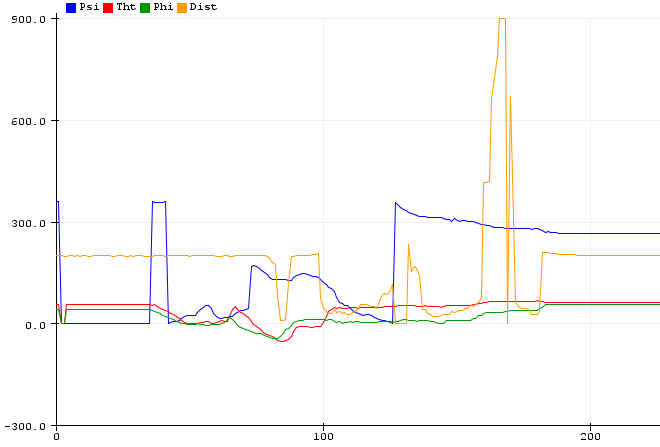
\includegraphics[width=0.7\textwidth]{./Images/serial-plotter.png}
	\caption{\label{fig:euler-test}Euler Angles Test}
\end{figure}

%\begin{figure}[H]
%	\centering
%	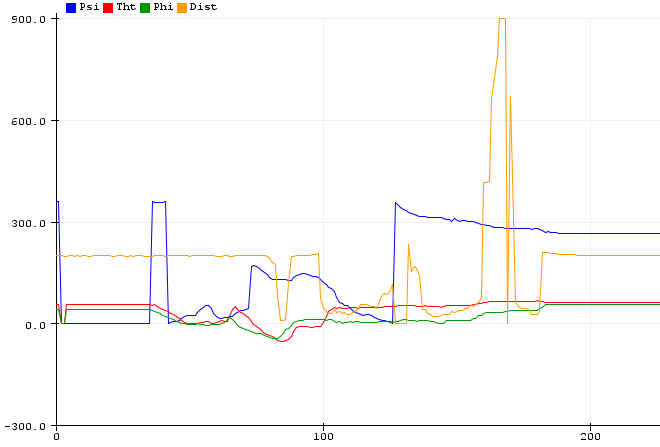
\includegraphics[width=0.7\textwidth]{./Images/serial-plotter.png}
%	\caption{\label{fig:range-test}Sensor Ranging Test}
%\end{figure}

\noindent It follows then, that we can define a range grid in polar coordinates where the maximum range detected is plotted versus yaw angle of the rollator. In this plot, we can also see precisely when there is an obstacle that causes a reduction in range.\\

% object identification test - classify obstacles and send walker into a moded resposne
% relay audio feedback to user informing them what is ahead
\subsubsection{Identification Importance}
The tiers of testing goals are:
\begin{enumerate}
	\item \textbf{Basic:} Alert the network there is a certain type of obstacle present (i.e. person, dog, car).
	\item \textbf{Stretch:} Alert the network that if two or more cars are present, "road ahead." If two or more people are present, "crowd ahead." Rank how urgent the situation is.
	\item \textbf{Advanced:} If range sensors return low but no obstacles classified, alert the network "wall." This is a placeholder code for any static solid obstacle.
\end{enumerate}

% object avoidance test - activate feedback and update motor speeds
\subsubsection{Control Feedback}
A successful control feedback test is defined by:
\begin{enumerate}
	\item \textbf{Basic:} Successfully vibrate the rollator handlebars via the haptic motors attached.
	\item \textbf{Stretch:} Increase the frequency of vibration as range reading decreases.
	\item \textbf{Advanced:} Spatially aware haptic feedback - left and right handlebars indicate the location of the obstacle.
\end{enumerate}

% in SD2, will need to refine turning ratios, hazard range thresholds, and work on stretch requirements.
\subsection{System Integration, Testing, and Evaluation}
\noindent System integration was already incorporated to some extent into the subsystem testing described in the previous subsection. However, there will be further concerns and scrutiny the FORWARD system must be subjected to as a whole. Among basic properties such as secure mounting and housing in the electronics chassis (discussed in section \ref{chassis}), it is good to consider waterproofing, temperature, viability with low battery/power supply, and configurations with sensors on, camera off, or vice versa. This should be done in order to ensure a reliable product is brought to the user.\\

\noindent \underline{\textit{PCB Assembly and Testing}}
\noindent As mentioned, the printed circuit board should be tested with varying levels of battery life remaining. \\

\noindent \underline{\textit{Determining and tuning motor coefficients}} During integration, it will be necessary to assign values governing the yaw steering command to the speed of the motors and haptic feedback signals. There should exist some constants that taking into account the rollator dynamics, can be calculated to scale the motors in order to achieve the desired turning angle. Additionally, once integration has been achieved, these scalars can be fine-tuned to optimize the rollator performance response.\\

\noindent \underline{\textit{Autonomous Navigation with Cooperative User}}
\noindent With motors installed on the rollator, which is also equipped with GNC software, there should be decision-making in the main code to distinguish how FORWARD adapts based on the environment. Some scenarios that come to mind are:
\begin{enumerate}
	\item Evasive mode. FORWARD takes full control (i.e. emergency stop)
	\item Cooperative navigation mode. FORWARD guides the user in a way does not infringe on their free movement.
	\item Dormant mode. User has full control of direction. \footnote{This is distinct from system powered off because the electronics are still in operation, they are just not being stimulated from the environment in a way that demands response from FORWARD}
\end{enumerate}
This step is probably the most difficult to implement at the same time as PCB development, motor coefficient tuning, and critical design review are taking place. Oftentimes, system moding is not as straightforward as it is cut out to be; in the boundary conditions when FORWARD will transition from one mode to the next, the team will have to carefully design the GNC software to remain stable. In other words, it remains subjective exactly when to apply emergency braking or how to define edge cases of multi-obstacle scenarios. Curb lifting, headlights in lowlight environments, and the other advanced requirements also remain undefined at this time.\\

\noindent \underline{\textit{Free Roam Evaluation}}
\noindent The final phase of testing is done when FORWARD integration is complete, and this is called the free roam evaluation. Essentially, the walker will be driven out in public for a pre-determined period of time, and the team will note mishaps and incidents that the guidance, navigation, and control protocols fail to prevent. These would be noted for future improvements for future endeavors and projects or products. This evaluation method will truly test and determine the successful or unsuccessful implementation of FORWARD from the beginning specifications and requirements listed. Multi-obstacle scenarios, mixtures of incline and decline territories, and mild levels of danger will be encountered. If requirements are met, design is up to specification, and all previous tests have been passed, we are confident FORWARD evaluation will be a success.\\